\documentclass[12pt]{article}
\usepackage{geometry} 
\geometry{letterpaper}
\usepackage{graphicx}
%\usepackage{Sweave}
%\setcounter{secnumdepth}{-2}

% \VignetteIndexEntry{How to use the ss3sim package to run simulations in SS3}
% \VignetteKeyword{metapopulations}
% \VignetteKeyword{ecology}

%\usepackage[round]{natbib} 
%\bibliographystyle{apalike}   
%\bibpunct{(}{)}{;}{a}{}{;}   

\title{How to use the \texttt{ss3sim} package to run\\simulations in \texttt{SS3}}
\author{Sean C. Anderson, \ldots}
\date{}

\begin{document}
\maketitle

\section{Installing the \texttt{ss3sim} \texttt{R} package}

The package can be installed and loaded with:

\begin{verbatim}
# install.packages(c("r4ss", "MCMCpack")) # dependencies, if needed
# install.packages("devtools")
# devtools::install_github("ss3sim", username="seananderson")
library(ss3sim)
\end{verbatim}

\noindent
While the package is under active development, it's a good idea to install a 
new version every day or so using the \texttt{install\_github} command:

\begin{verbatim}
devtools::install_github("ss3sim", username="seananderson")
\end{verbatim}

\noindent
You can read the help files and access this vignette again with:

\begin{verbatim}
help(package = "ss3sim")
vignette("ss3sim")
\end{verbatim}

\noindent
Note that you can install the development version of the package with:

\begin{verbatim}
devtools::install_github("ss3sim", username="seananderson", ref="develop")
\end{verbatim}

\noindent
The development version may contain recent and untested changes.

\section{Putting \texttt{SS3} in your path}
\texttt{SS3} must be in your path for the \texttt{ss3sim} package to work. Your 
``path'' is a list of folders that your operating system looks in whenever you 
type the name of a program on the command line. Having a binary in your path 
means that your operating system knows where to look for the file regardless of 
what folder you're working in. 

\subsection{For Unix (Linux and OS X)}
To check if \texttt{SS3} is in your path: open a Terminal window and type 
\texttt{which SS3} and hit enter. If you get nothing returned then SS is not in 
your path. The easiest way to fix this is to move the \texttt{SS3} binary to a 
folder that's already in your path. To find existing path folders type 
\texttt{echo \$PATH} in the terminal and hit enter. Now move the \texttt{SS3} 
binary to one of these folders. For example, in a Terminal window type:

\begin{verbatim}
  sudo cp ~/Downloads/SS3 /usr/bin/
\end{verbatim}

\noindent
You will need to use \texttt{sudo} and enter your password after to have 
permission to move a file to a folder like \texttt{/usr/bin/}.

If you've previously modified your path to add a non-standard location for the 
\texttt{SS3} binary, you may need to also tell \texttt{R} about the new path. 
The path that \texttt{R} sees may not include additional paths that you've 
added through a configuration file like \texttt{.bash\_profile}. You can add to 
the path that \texttt{R} sees by including a line like this in your 
\texttt{.Rprofile} file. (This is an invisible file in your home directory.)

\begin{verbatim}
Sys.setenv(PATH=paste(Sys.getenv("PATH"),"/my/non-standard/folder",sep=":")) 
\end{verbatim}

\subsection{For Windows}
To check if SS is in your path: open a DOS prompt and type \texttt{ss3 -?} and 
hit enter. If you get a line like ``ss3 is not recognized \ldots'' then SS is 
not in your path. To add it to your path:

\begin{enumerate}
  \item Find the latest version of the \texttt{ss3.exe} binary on your computer
  \item Record the folder location. E.g. \texttt{C:/SS3.24o/}
  \item Click on the start menu and type ``environment''
  \item Choose ``Edit environment variables for your account'' under Control 
    Panel
  \item Click on \texttt{PATH} if it exists, create it if doesn't exist
  \item Choose \texttt{PATH} and click edit
  \item In the ``Edit User Variable'' window add to the \textbf{end} of the 
    ``Variable value'' section a semicolon and the \texttt{SS3} folder location you 
    recorded earlier. E.g. \texttt{;C:/SS3.24o/}
  \item Restart your computer
  \item Go back to the DOS prompt and try typing \texttt{ss3 -?} and hitting 
    return again.
\end{enumerate}


\section{Setting up the file structure}
This package is set up assuming that you have an established base case 
operating model and estimation model to work with. Each operating model and 
estimation model should be in their own folder. The operating model folder 
should have the files:

\begin{verbatim}
yourmodel.ctl
yourmodel.dat
ss3.par
starter.ss
forecast.ss
\end{verbatim}

\noindent
The estimation model folder should have:

\begin{verbatim}
yourmodel.ctl
yourmodel.dat # optional; not used
starter.ss
forecast.ss
\end{verbatim}

\noindent
In both cases, nothing more and nothing less. The names of the \texttt{.ctl} 
and \texttt{.dat} files are not important. The package functions will rename 
them after they are copied to appropriate folders. These files should be 
derived from the \texttt{.ss\_new} files but named as listed above. It's 
important to use these \texttt{.ss\_new} files so they have consistent 
formatting. Many of the functions in this package depend on that formatting.

For the purposes of the Fish 600 project, we have unique case identifiers which 
combine to create unique scenarios. The types of cases are: natural mortality 
(M), fishing mortality (F), data quality (D), and retrospective (R). And the 
species are cod (cod), sardine-like (sar), and flatfish (fla). It's important 
to use these three letter abbreviations for the species since the functions 
assume that the last three letters represent a species (or some other 
identifier for a different project).

The different version of each case are identified with numbers. So, for 
example, the base case scenario for cod is identified as 
\texttt{M1-F1-D1-R1-cod}. We will have a spreadsheet that describes each of 
these in plain language.

The function \texttt{copy\_ss3models} creates a folder structure and copies 
over the operating and estimation models. The folder structure looks like:

\begin{verbatim}
  M1-F1-D1-R1-cod/1/om
  M1-F1-D1-R1-cod/1/em
  M1-F1-D1-R1-cod/2/om
  M1-F1-D1-R1-cod/2/em
  ...
\end{verbatim}

\noindent
If you are using bias adjustment (\texttt{bias\_adjust = TRUE}) then there 
will be some additional folders. In that case the folders will look like:

\begin{verbatim}
  M1-F1-D1-R1-cod/bias/1/om
  M1-F1-D1-R1-cod/bias/1/em
  M1-F1-D1-R1-cod/bias/2/om
  M1-F1-D1-R1-cod/bias/2/em
  ...
  M1-F1-D1-R1-cod/1/om
  M1-F1-D1-R1-cod/1/em
  M1-F1-D1-R1-cod/2/om
  M1-F1-D1-R1-cod/2/em
  ...
\end{verbatim}

\noindent
Note that the operating and estimating model folders have been renamed
\texttt{om} and \texttt{em} within each iteration, the operating and estimation 
models have been checked to make sure they contain the minimal files (as listed 
above), the filenames have been made all lowercase, the data file has been 
renamed \texttt{data.dat}, the control files have been renamed \texttt{om.ctl} 
or \texttt{em.ctl}, and the starter and control files have been adjusted to 
reflect these new file names.

The functions in this package assume you've set your working directory in 
\texttt{R} to be the base folder where you will store the scenario folders.

\section{Creating the input configuration files}
You will need to have a folder containing ``case'' argument definitions. These 
plain text files are read by \texttt{get\_caseval} and turned into argument 
lists that are passed to \texttt{run\_ss3sim}. You can create template input 
files by running \texttt{create\_argfiles}. It reads the various functions and 
parses the arguments and default values into plain text files. The default 
settings create these files:

\begin{enumerate}
  \item \texttt{M0-spp.txt}
  \item \texttt{F0-spp.txt}
  \item \texttt{index0-spp.txt}
  \item \texttt{agecomp0-spp.txt}
  \item \texttt{lcomp0-spp.txt}
  \item \texttt{R0-spp.txt} 
  \item \texttt{S0-spp.txt} 
  \item \texttt{G0-spp.txt} 
  \item \texttt{E0-spp.txt} 
\end{enumerate}

Look in your working directory for the template files. Change the case ID 
number (defaults to \texttt{0}) and the species identifier to a three letter 
identifier. For the Fish 600 project use one of \texttt{cod}, \texttt{sar}, or 
\texttt{fla} for cod, sardine, or flatfish. An example filename would be 
\texttt{M1-sar.txt} or \texttt{lcomp2-fla.txt}. The case \texttt{D1} 
corresponds to the files \texttt{index1-spp.txt}, \texttt{agecomp1-spp.txt}, 
and \texttt{lcomp0-spp.txt}. The other case types have single argument files.

The first column in the text files denotes the argument to be passed to a 
function. The second argument denotes the value to be passed. You can use any 
simple \texttt{R} syntax. For example: \texttt{c(1, 2, 4)}, or \texttt{seq(1, 100)} or 
\texttt{1:100} or \texttt{matrix()}. Character objects don't need to be quoted, 
but can be if you'd like. However, be careful not to use the delimiter (set up 
as a semicolon) anywhere else in the file besides to denote columns. You can 
add comments after any \texttt{\#} symbols. Internally, the functions evaluate 
in \texttt{R} any entries that have no character values (e.g. \texttt{1:100}) or have an 
alpha-numeric character followed by a \texttt{(}. Anything that is character 
only or has character mixed with numeric but doesn't have the regular 
expression \texttt{"[A-Za-z0-9]("} gets turned into a character argument.

Putting that all together, here's what an example \texttt{F1-cod.txt} file 
might look like:

\begin{verbatim}
years; 1:100
years_alter; NA 
fvals; NA
\end{verbatim}

\section{Running the models}

The \texttt{run\_ss3sim} function is a wrapper function. It adjusts the natural 
mortality, adjusts the fishing mortality, adds recruitment deviations, calls 
\texttt{run\_ss3model} to run the operating model, samples various survey 
estimates from the operating model, changes the age composition data as 
specified, changes the length composition data as specified, copies and renames 
files as necessary, and calls \texttt{run\_ss3model} again to run the 
estimation model.

The \texttt{run\_fish600} function is a higher-level wrapper that deals with 
parsing the case input files and then passes these arguments on to 
\texttt{run\_ss3sim}. This is what we will use for the Fish 600 project.

Say you have your input case files setup and you want to run the first 
iteration of the scenario \texttt{M1-F1-D1-R1-cod}. You could run it like this:

\begin{verbatim}
# First grab the example package data:
d <- system.file("extdata", package = "ss3sim")
f <- paste0(d, "/run_ss3sim_eg/")
om_model_dir <- paste0(f, "cod_om")
em_model_dir <- paste0(f, "cod_em")
case_folder <- paste0(f, "case-arguments")

# Without bias adjustment:
run_fish600(iterations = 1, scenarios = c("M1-F1-D1-R1-E1-S1-G1-cod"),
case_folder = case_folder, om_model_dir = om_model_dir,
em_model_dir = em_model_dir)

# With bias adjustment:
# (Note that bias_nsim should be bigger, say 5, but it is set to 2
# here so the example runs faster.)
run_fish600(iterations = 1, scenarios = c("M1-F1-D1-R1-E1-S1-G1-cod"),
case_folder = case_folder, om_model_dir = om_model_dir,
em_model_dir = em_model_dir, bias_adjust = TRUE,
bias_nsim = 2)
\end{verbatim}

See the PDF version of this vignette for a flow chart illustrating how 
\texttt{run\_fish600} and \texttt{run\_ss3sim} work:

\begin{verbatim}
vignette("ss3sim")
\end{verbatim}

\begin{figure}[htbp]
  \centering
    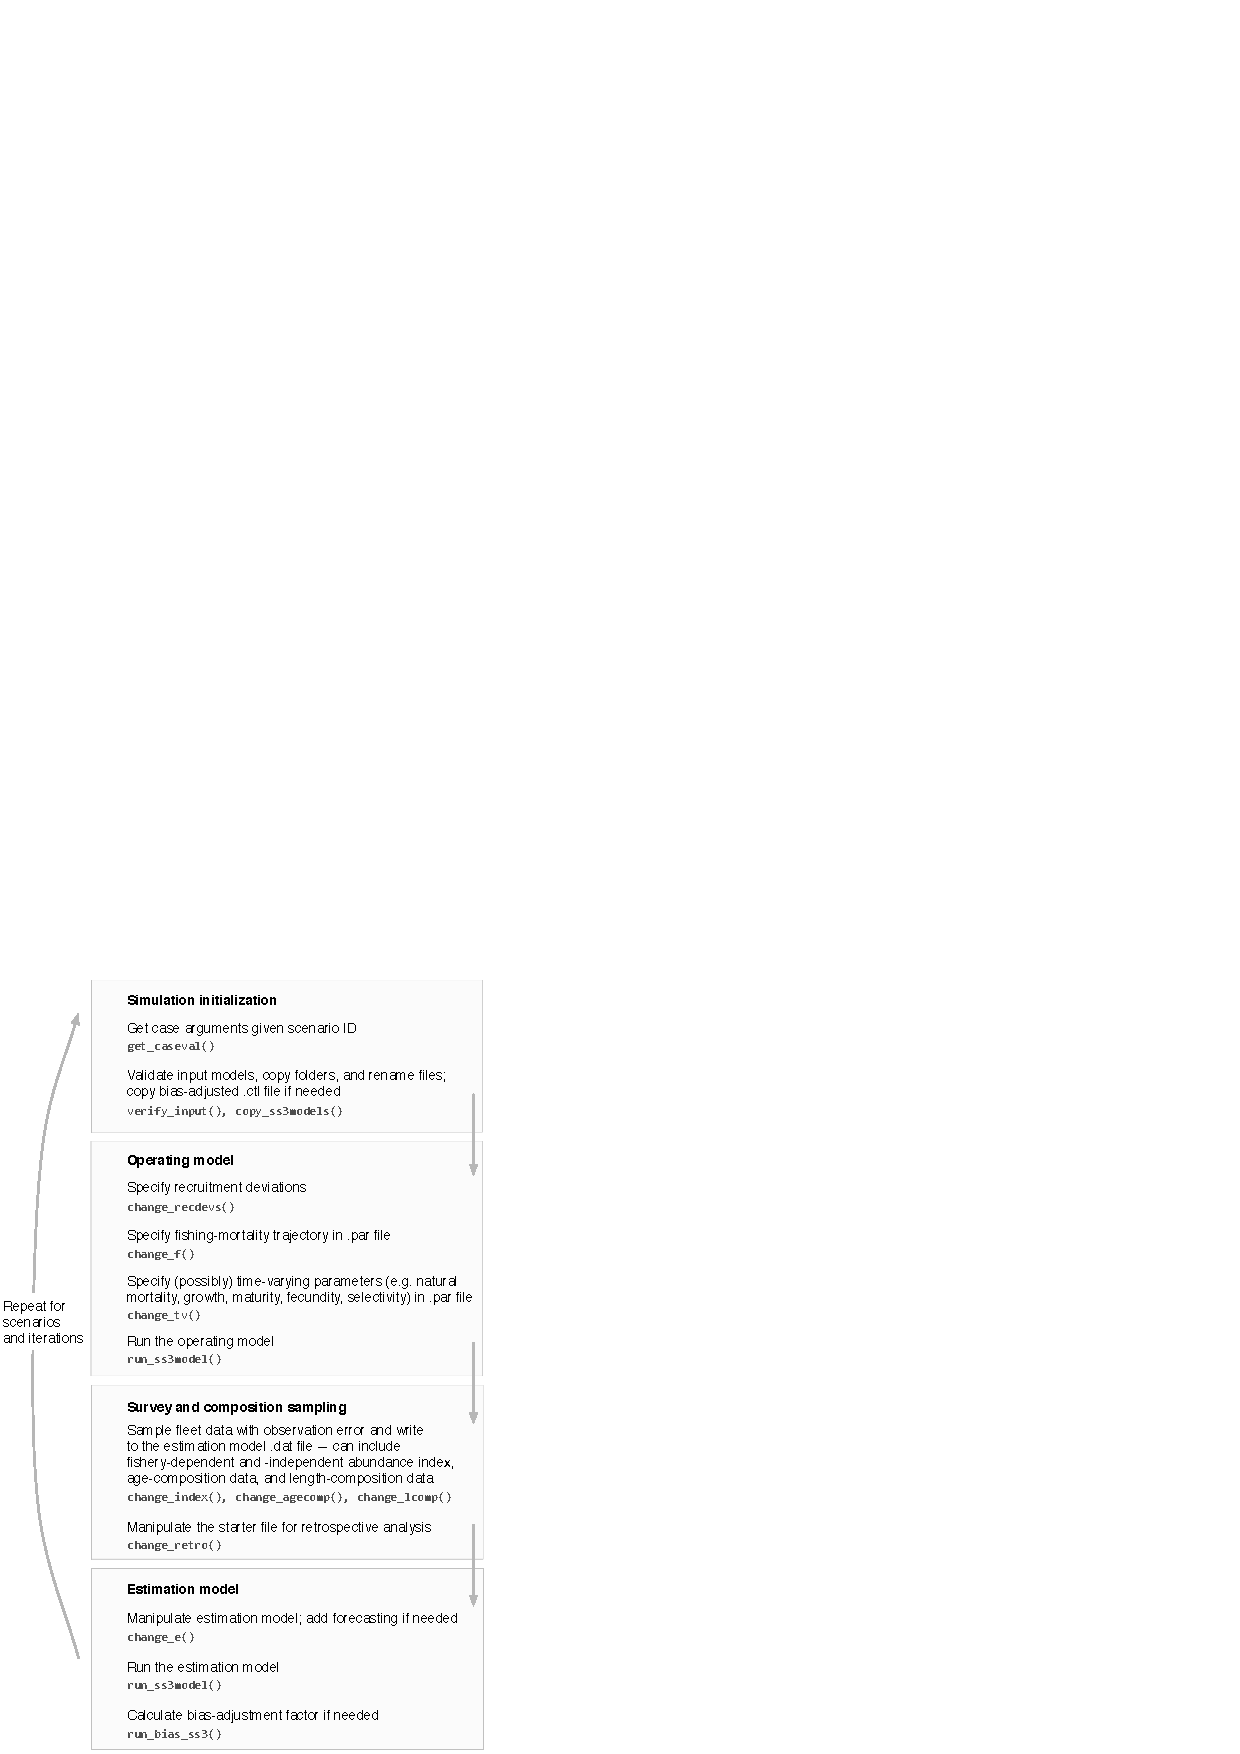
\includegraphics[width=5.5in]{sim-steps.pdf}
  \caption{Simulation steps. Higher-level function calls are shown on the 
    right.}
  \label{fig:sim-steps}
\end{figure}

\end{document}
